% Created 2017-09-28 Thu 07:45
\documentclass[11pt]{article}
\usepackage[utf8]{inputenc}
\usepackage[T1]{fontenc}
\usepackage{fixltx2e}
\usepackage{graphicx}
\usepackage{longtable}
\usepackage{float}
\usepackage{wrapfig}
\usepackage{rotating}
\usepackage[normalem]{ulem}
\usepackage{amsmath}
\usepackage{textcomp}
\usepackage{marvosym}
\usepackage{wasysym}
\usepackage{amssymb}
\usepackage{hyperref}
\tolerance=1000
\date{Sept 25-29, 2017}
\title{Week 5 lecture notes - PSYC 3330}
\hypersetup{
  pdfkeywords={},
  pdfsubject={},
  pdfcreator={Emacs 25.2.1 (Org mode 8.2.10)}}
\begin{document}

\maketitle
So far this semester, we have used statistics to \textbf{describe} data.  Now, we will begin using statistics as an \textbf{inference tool}.  To do this, we need to discuss \textbf{probability}.

\section*{Definition}
\label{sec-1}

Suppose we have a list of possible \emph{outcomes}, labeled A, B, C, D, and so on.  Then:

\[
p(A) = \text{ "the probability of A" }=\frac{\text{number of outcomes classified as A}}{\text{total number of possible outcomes}}
\]

Example: What is the probability of picking a king of spades from a standard deck of 52 cards?

Answer:

\[
p(\text{king of spades}) = \frac{\text{# of times king of spades appears}}{\text{number of cards in the deck}} = \frac{1}{52}
\]

Example: What is the probability of picking a heart from a deck?

Answer:

\[
p(\text{heart}) = \frac{\text{# hearts in a deck}}{\text{number of cards in the deck}} = \frac{13}{52} =\frac{1}{4} = 0.25
\]

\section*{Probability distributions}
\label{sec-2}

The more common way we will encounter probability is as part of a \emph{probability distribution}.

Example: Suppose we have 40 slips of paper, each labeled with one of the numbers 1,2,3,4,5.  Specifically, assume they are labeled with the following frequencies:

\begin{center}
\begin{tabular}{rr}
X & f\\
\hline
5 & 2\\
4 & 10\\
3 & 16\\
2 & 8\\
1 & 4\\
\end{tabular}
\end{center}

If we compute the \emph{relative frequencies} (as percentages of the total frequency), we get the following:

\begin{center}
\begin{tabular}{rrr}
X & f & p\\
\hline
5 & 2 & 0.05\\
4 & 10 & 0.25\\
3 & 16 & 0.40\\
2 & 8 & 0.20\\
1 & 4 & 0.10\\
\end{tabular}
\end{center}

Visually, this distribution looks like the following graph:

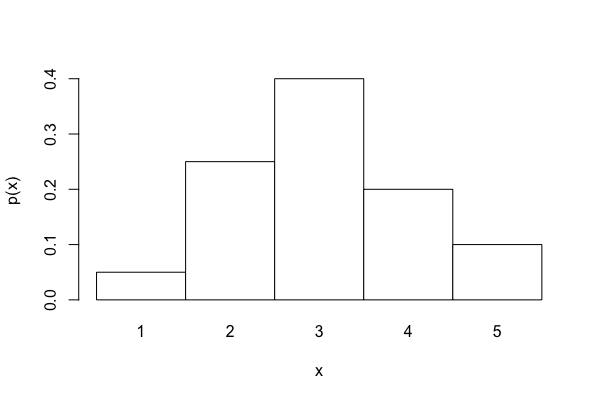
\includegraphics[width=.9\linewidth]{figures/week5/plot1.png}

This graph represents the \emph{probability distribution}.  Essentially, it tells us everything we would want to know about this particular situation.  For example, suppose our task is to randomly select a slip of paper.  We can then ask lots of questions, such as:

\begin{itemize}
\item What is the probability of selecting a 3?
\begin{itemize}
\item Answer: $p(3) = 0.40$
\end{itemize}
\item What is the probability of selecting a 5?
\begin{itemize}
\item Answer: $p(5) = 0.05$
\end{itemize}
\end{itemize}

We can also ask more complex questions:

\begin{itemize}
\item What is the probability of selecting a slip of paper with a value greater than 2?
\begin{itemize}
\item Answer: $p(x>2) = 0.40 + 0.25 + 0.05 = 0.70$
\end{itemize}
\end{itemize}

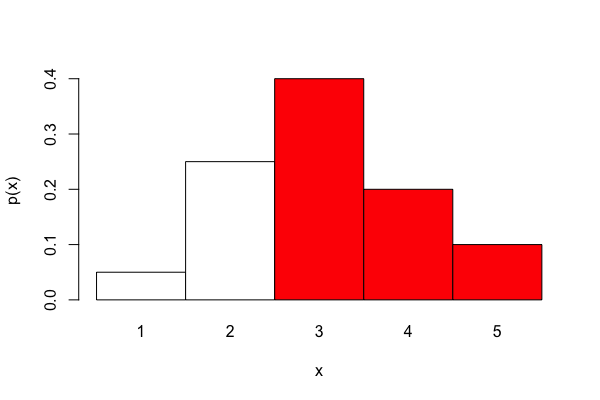
\includegraphics[width=.9\linewidth]{figures/week5/plot2.png}

\begin{itemize}
\item What is the probability of selecting a slip of paper with a value less than 5?
\begin{itemize}
\item Answer: $p(x<5) = 0.10 + 0.20 + 0.40 + 0.25 = 0.95$
\end{itemize}
\end{itemize}

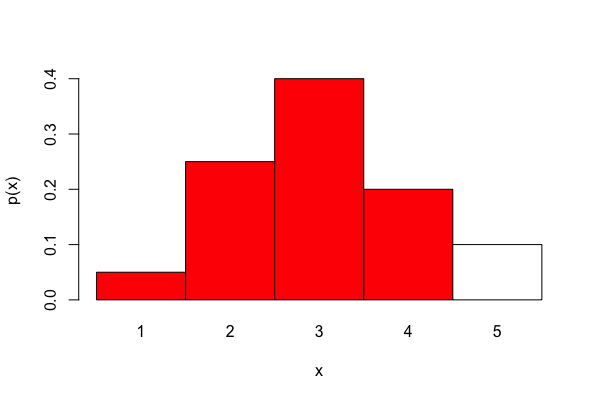
\includegraphics[width=.9\linewidth]{figures/week5/plot3.png}

\begin{itemize}
\item What is the probability of selecting a value greater than 1 and less than 4?
\begin{itemize}
\item Answer: $p(1 < x < 4) = 0.20 + 0.40 = 0.60$
\end{itemize}
\end{itemize}

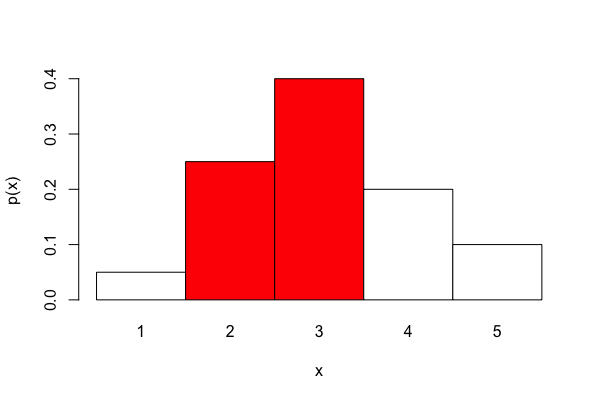
\includegraphics[width=.9\linewidth]{figures/week5/plot4.png}  

\section*{The normal distribution}
\label{sec-3}

The probability distribution that we will use quite a bit this semester is known as the \emph{normal distribution}.  It is defined by the following equation:

\[
f(x) = \frac{1}{\sqrt{2\pi\sigma^2}}e^{\frac{-(x-\mu)^2}{2\sigma^2}}
\]

where $\mu$ is the mean and $\sigma$ is the standard deviation.

More importantly for us, it looks like the following:

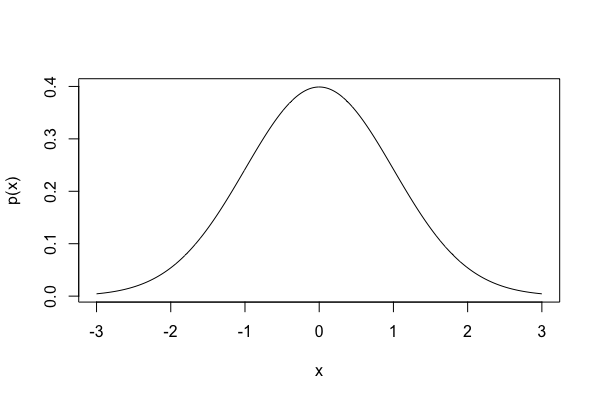
\includegraphics[width=.9\linewidth]{figures/week5/normal.png}

Technically, this curve depends on $\mu$ and $\sigma$.  However, if we transform to $z$-scores, we can use ONE standardized distribution, known as the \emph{standard normal distribution}.

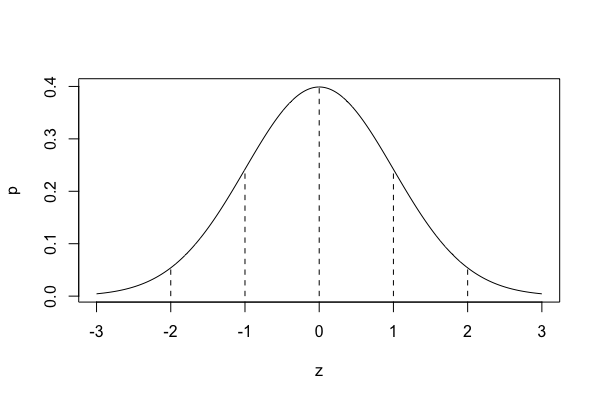
\includegraphics[width=.9\linewidth]{figures/week5/zCurve.png}

We know lots of things about the standard normal curve:
\begin{itemize}
\item it is unimodal and symmetric
\item 34\% of the distribution lies within one standard deviation of the mean
\end{itemize}
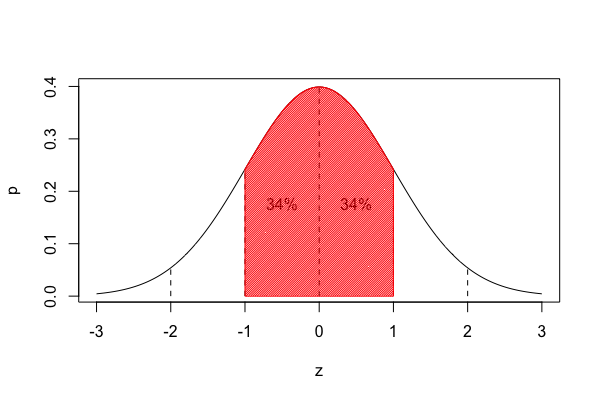
\includegraphics[width=.9\linewidth]{figures/week5/oneSD.png}

\begin{itemize}
\item 95\% of the distribution lies within two standard deviations of the mean
\end{itemize}
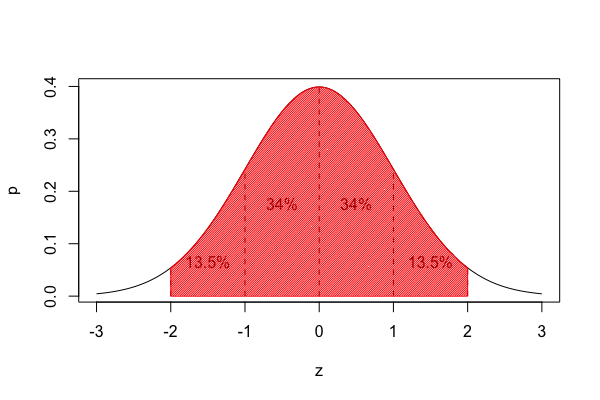
\includegraphics[width=.9\linewidth]{figures/week5/twoSD.png}


This is helpful.  For example, consider that IQ scores are normally distributed with mean $\mu=100$ and standard deviation $\sigma=15$.  Then we know the following:

\begin{itemize}
\item 68\% of the population scores between 85 and 115
\item 95\% of the population scores between 70 and 130
\item 2.5\% of the population scores above 130
\item 2.5\% of the population scores below 70
\end{itemize}


In fact, we can modify this to have a nice "intuitive" rule for probabilities under the normal curve:

\subsection*{50-34-14 rule:}
\label{sec-3-1}
\begin{itemize}
\item 50\% of the curve is above the mean
\item 34\% of the curve is between the mean and 1 SD
\item 14\% of the curve is between 1 SD and 2 SD
\end{itemize}

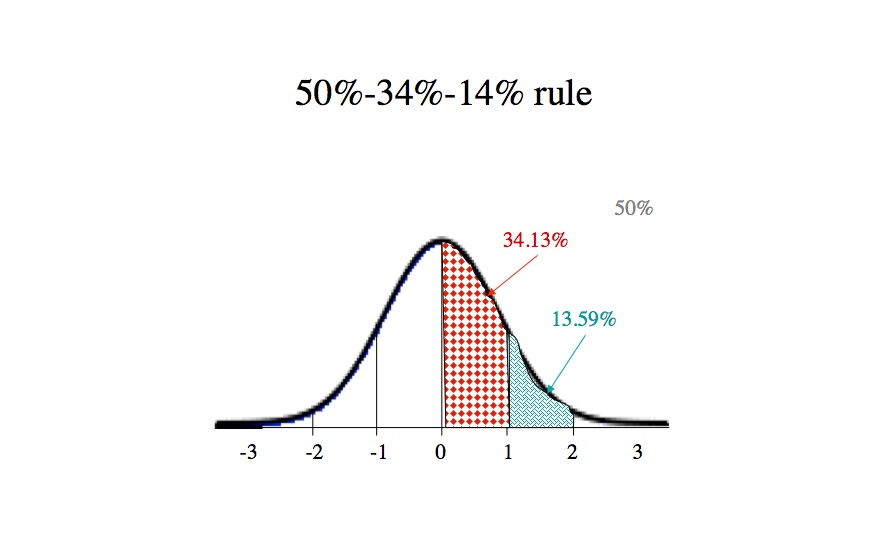
\includegraphics[width=.9\linewidth]{figures/week5/50-34-14.jpeg}

Examples:
\begin{itemize}
\item suppose a data set is normally distributed with $\mu=40$ and $\sigma=5$.  Use the 50-34-14 rule to approximate the percentage of that data that is:
\begin{itemize}
\item above 45
\item above 30
\item above 35
\item below 40
\item below 45
\item below 30
\item below 35
\end{itemize}

\item suppose a data set is normally distributed with $\mu=45$ and $\sigma=6$.  Use the 50-34-14 rule to approximate the minimum score needed for a data point to be in the top:
\begin{itemize}
\item 2\%
\item 16\%
\item 50\%
\end{itemize}
\end{itemize}


To make more exact computations, we will need to learn how to use the \emph{unit normal table}.  You can download one on our blackboard site, or use the one in the back of your textbook.

\section*{Using the unit normal table}
\label{sec-4}

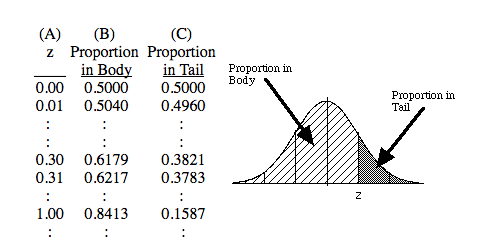
\includegraphics[width=.9\linewidth]{figures/week5/table.png}

\begin{itemize}
\item Column A: the $z$ score
\item Column B: probability of being LESS than $z$ (proportion in \textbf{body})
\item Column C: probability of being GREATER than $z$ (proportion in \textbf{tail})
\end{itemize}

Finding probabilities:

\begin{enumerate}
\item sketch the normal distribution, showing the mean \& standard deviation
\item sketch the score in question, being sure to place it on the correct side of the mean and roughly the correct distance from the mean
\item decide if you need the probability of getting a score GREATER or LESS. Shade this area on your sketch.
\item translate the X score into a Z-score
\item Use the correct column (and sign) to find the probability in the unit normal table.
\end{enumerate}

Example:  Recall that IQ scores are normally distributed with $\mu=100$ and $\sigma = 15$. 
\begin{itemize}
\item What is the probability of having an IQ of 125 or above?
\item What is the probability of having an IQ of 80 or less?
\end{itemize}


Another type of problem: finding scores required for a certain probability:

Example: what IQ score do you need in order to be in top 5\% of population?

Steps:
\begin{enumerate}
\item sketch the normal distribution
\item shade the region corresponding to the required probability
\item locate the probability in the correct column of the table
\item label the edge of the shaded region with the z-score from the table
\item compute the corresponding raw score.
\end{enumerate}

For this example, note that the upper tail is needed.  So, we need to find p=0.05.  From the table, this tells us z=1.65.  So, $X=M+Z\cdot SD = 100 + 1.65(15)=124.75$.

Final example: On a particular test, assume that $\mu=50$ and $\sigma=10$.  If a person is in the bottom 30\% of the class on this test, what is the highest score the person could have scored?
% Emacs 25.2.1 (Org mode 8.2.10)
\end{document}